\subsection{Compass Data Processing}
Once the Zynq7 Processing System was re-customized to support communication with the PmodNAV, the Xilinx SDK was relaunched. All of the magnetometer's data was processed in the Programmable Software on the ARM Processor to rotate the rangefinder's data according to the sensor suite's compass heading.

\subsubsection{Programmable Software}
The SPI communication in the SDK was implemented by following example code provided within the SPIPS driver in the Xilinx SDK. The examples are located in the following folder: \path{C:\Xilinx\SDK\2016.2\data\embeddedsw\XilinxProcessorIPLib\drivers\spips_v3_0\examples\}.
\par
By following Xilinx's examples, the magnetometer initialization and communication from Section \ref{imu_settings} was implemented. In the programmable software, the axis data was read into an unsigned 8-bit variable. The data points were rearranged and then stored into a buffer of type $int$ for each axis. The magnetometer's axis data was signed and expressed in Two's Complement format \cite{lsm9ds1}.\footnote{ Two's Complement is a way of encoding signed numbers in binary where the most significant bit is used as a sign bit, with '1' signifying a negative number and '0' signifying a positive number. To convert a positive number to negative, all of the bits are inverted and then 1 is added to the resultant number \cite{2sComp}.} Combining a data point in this manner works if the $int$ data type were only 16 bits. However, the data type $int$ in the Xilinx SDK is 32 bits. For positive numbers this method was sufficient, but for negative numbers this process dropped the sign bit. The sign bit was the most significant bit of the axes' 16-bit data, which got lost when getting stored in a 32-bit integer. This problem was corrected by checking each data point's sign bit. If each data point was greater than or equal to 8000\textsubscript{16} then the sign bit must be '1', indicating a negative number. If necessary, the data was turned negative by subtracting FFFF\textsubscript{16} and adding 1.
\par
To perform the necessary complex math on the data, the header file $math.h$ was linked and included into the project. This was done by right clicking on the application project, choosing Properties $\rightarrow$ C/C++ Build $\rightarrow$ Settings $\rightarrow$ Tool Settings $\rightarrow$ ARM v7 gcc linker $\rightarrow$ Libraries, and then adding $m$ under the Libraries (-l) section, shown in Figure \ref{including_math}. In addition, $math.h$ still was included by using $\#include$ in the project's source code file.

\begin{figure}[H]
	\centerline{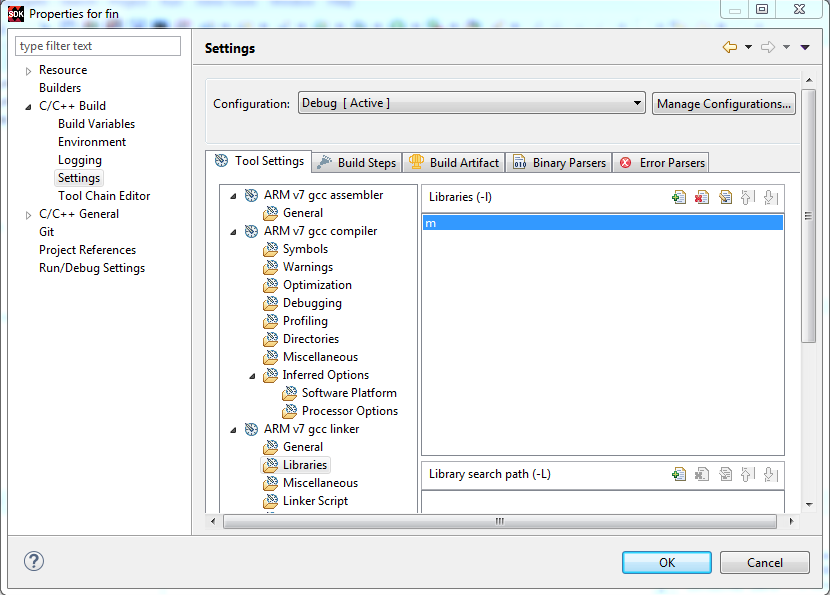
\includegraphics[width=1\textwidth]{including_math.png}}
	\caption{Linking $math.h$ into the Application Project}
	\label{including_math}
\end{figure}

The complex math was used to convert the magnetometer's axis data, in terms of milligauss per bit, to a compass heading in degrees. The equation that was used for this transformation is shown in Equation \ref{GaussToDegrees}. Note that the arctangent function from $math.h$ outputs data in radians, so the resultant angle was multiplied by $\dfrac{180}{\pi}$ to convert it to degrees.

\begin{equation}
	\textrm{Compass Heading} = \arctan(\dfrac{y}{x})\times\dfrac{180}{\pi}
	\label{GaussToDegrees}
\end{equation}

To convert the compass heading to a rangefinder step offset, Equation \ref{CompassHeadingToStepOffset} was used. This calculation was possible because there were a total of 768 rangefinder steps around the rangefinder's 270$^\circ$ field of vision \cite{urg04lx_datasheet}.

\begin{equation}
	\textrm{Step Offset} = \dfrac{\textrm{Compass Heading}}{\dfrac{360^\circ}{1024\ steps}}
	\label{CompassHeadingToStepOffset}
\end{equation}

The resultant step offset was added to the rangefinder's step in order to account for the sensor suite's compass direction deviation from North. When the sensor suite faced due North the step offset equated to 0, so the rangefinder's data was not rotated. When the ZedBoard faced due South the step offset equated to 512, which rotated the rangefinder data by $180^\circ$.






